% Include after \usepackage{graphicx} in an IEEEtran manuscript.
% Paths assume this file and output/ are copied beside the main manuscript.
\section{Experimental Results}
\label{sec:experiments}

\subsection{Experimental Setup and Aggregation}
The evaluation uses the existing default benchmark measurements, comprising
162 parameter--seed cases and 1,458 timed executions. The task counts are
$n\in\{100,500,1000\}$, the server counts are $m\in\{25,100\}$, and eligibility
probabilities are $p\in\{0.01,0.1,0.5\}$. Each potential task--server pair is
independently eligible with probability $p$. The observed number of eligible
pairs, denoted by $r$, is retained in the analysis rather than replaced by
its expectation $pnm$. Three capacity distributions are evaluated: fixed
capacity four; discrete uniform capacity on $\{0,\ldots,8\}$; and skewed
capacity equal to 40 with probability 0.1 and zero otherwise. All have
expected capacity four per server, but their realized total capacities differ.
Seeds 11, 29, and 47 define three instances per parameter setting. For each
seed, eligibility graphs are shared across capacity distributions.

The recorded environment is OpenJDK 17.0.19 on macOS 26.1, with an aarch64
architecture, 10 available processors, and a fixed 512-MiB initial and maximum
Java heap. The available data contain one JVM process. Each case has five
discarded warm-up executions and nine measured executions using fresh residual
networks and \texttt{System.nanoTime()}~\cite{oracleNanoTime}. This API reports
elapsed-time differences in nanoseconds, but does not guarantee nanosecond
resolution. Construction includes allocation of
residual edges and Dinic work arrays. Total time includes construction, maximum
flow, and assignment extraction; input generation, validation, and CSV output
are excluded.

Each instance is represented by its median over nine repetitions. Unless
otherwise stated, plotted central values are medians of these instance medians
over the three seeds. Error bars span the minimum and maximum seed medians;
they are descriptive ranges, not confidence intervals. Edge-count plots show
individual instance medians at their actual $r$ values. All timing coordinates
come from the recorded measurements. Connecting segments indicate sampled
trends and do not represent additional observations. Logarithmic runtime axes
accommodate the measured dynamic range. Reported values are rounded for
presentation.

\subsection{Task Count and Eligibility Edges}
Figure~\ref{fig:tasks} controls the server count at $m=100$ and uses fixed
capacity four. At $p=0.1$, increasing $n$ from 100 to 500 and 1,000 increases
median total time from 0.0184~ms to 0.1145~ms and 0.2411~ms, respectively.
The corresponding Dinic times are 0.00517~ms, 0.0528~ms, and 0.1140~ms.
Thus, over the tenfold task-count increase, total time increases by a factor
of 13.12 and Dinic time by 22.06. These are finite-range growth factors;
three task counts do not establish an asymptotic empirical exponent.
Moreover, varying $n$ also changes the realized number of eligibility edges
and the attainable flow, despite holding $m$, $p$, and per-server capacity fixed.

Figure~\ref{fig:edges} fixes $n=1000$ and $m=100$ and plots time against
the measured eligibility edge count. Eligibility probability varies to produce
the different edge counts, so this is not an experiment that changes $r$
independently of graph topology. For fixed capacities, increasing $p$ from
0.01 to 0.5 increases the median observed $r$ from 1,014 to 50,116.
Median total time increases from 0.0870~ms to 1.3490~ms, and Dinic time
increases from 0.0606~ms to 0.5120~ms. Larger adjacency lists require
additional allocation and traversal even when the achievable assignment
cardinality changes little. These observations are consistent with such costs,
but do not independently identify their contribution.

\subsection{Server Count and Eligibility Density}
Figure~\ref{fig:servers} holds $n=1000$ and fixed per-server capacity four.
At $p=0.1$, increasing $m$ from 25 to 100 increases median total time from
0.1068~ms to 0.2411~ms and Dinic time from 0.0391~ms to 0.1140~ms.
This comparison changes both expected eligibility edge count and aggregate
server capacity; the median maximum flow increases from 100 to 400.
Only two server counts are available, which precludes a reliable determination
of the runtime growth law with respect to $m$.

Figure~\ref{fig:density} controls $n=1000$ and $m=100$. For fixed capacities,
median flow is 399 at $p=0.01$ and 400 at both $p=0.1$ and $p=0.5$.
Consequently, the substantial runtime increase at higher densities is accompanied
by almost no improvement in admitted tasks. Median flow for uniform capacities
is 392, 398, and 398 across these densities; for skewed capacities it is
77, 320, and 320. The skewed distribution is particularly constrained at low
density because many eligible edges lead to zero-capacity servers. At $p=0.01$,
its median total time is 0.0473~ms, compared with 0.0870~ms for fixed capacities.
This lower runtime is accompanied by fewer assigned tasks and should not be
interpreted as greater scheduling effectiveness. Realized median aggregate
capacities are 400, 398, and 320 for the fixed, uniform, and skewed distributions,
respectively; distribution comparisons therefore do not isolate capacity
concentration at an identical total capacity.

\subsection{Construction and Maximum-Flow Costs}
Figure~\ref{fig:components} separates network construction from maximum-flow
computation. At $n=1000$, $m=100$, and fixed capacities, construction increases
from 0.0250~ms at $p=0.01$ to 0.8224~ms at $p=0.5$; the corresponding
Dinic times are 0.0606~ms and 0.5120~ms. Thus, maximum-flow computation
dominates the component medians in this sparse setting, whereas construction
is larger in the dense setting. Across all 1,458 measured repetitions, the
median within-run construction, Dinic, and extraction fractions are 51.0\%,
47.0\%, and 1.8\%, respectively. These separately computed median fractions
need not sum to 100\%.

Construction is therefore a material cost in the observed implementation.
Forward/reverse edge objects and adjacency-list storage provide plausible
sources of allocation and memory-access overhead. Garbage collection, cache
behavior, and JVM compilation may also affect timings. The CSV files contain
no allocation, collection, cache, or phase-count counters, so these explanations
remain hypotheses rather than measured causal findings. An implementation
using compact edge arrays would require a separate controlled evaluation.

\subsection{Comparison with the Worst-Case Upper Bound}
The constructed network contains
\begin{equation}
V=n+m+2,\qquad E=n+m+r.
\end{equation}
Construction and extraction require $O(n+m+r)$ and $O(n+r)$ time,
respectively. Using Dinic's general $O(V^2E)$ bound, the complete algorithm
has worst-case upper bound
\begin{equation}
O\!\left((n+m+2)^2(n+m+r)\right),
\end{equation}
with $O(n+m+r)$ space. This is an upper bound rather than a tight runtime
prediction for the tested layered networks. In particular, $V^2E$ is an
operation-count expression without a calibrated conversion to elapsed time.

For the controlled slice $m=100$, $p=0.1$, and fixed capacities, median
$V^2E$ increases by factors of 41.04 and 274.19 as $n$ increases from
100 to 500 and 1,000. The corresponding measured total-time factors are
6.23 and 13.12, and Dinic-time factors are 10.22 and 22.06
(Fig.~\ref{fig:growth}). Observed growth is therefore much smaller than the
growth of this general worst-case expression over the measured range.
This is compatible with the upper bound: random instances need not require
the worst-case number of blocking-flow phases or edge traversals. Additionally,
fixed aggregate capacity caps flow at 400 in this slice even as the number
of tasks increases. The data do not establish which mechanism dominates.
No theoretical timing curve or synthetic timing observations are introduced.

\subsection{Limitations and Validity}
The results describe small synthetic instances, one JVM process, three input
seeds, three density values, and two server counts. Five warm-up executions
do not establish that JIT compilation stabilized. The distinction between
warm-up, steady-state measurement, and independent JVM invocations is
important in Java performance evaluation~\cite{georges2007}. Several intervals are only
a few microseconds long and may be sensitive to timer overhead, scheduling,
allocation, and background activity. CPU model, RAM, GC events, and per-phase
algorithm counters are not recorded. The measurements therefore do not
support hardware-independent performance claims, a statistical model of
process-level variability, or causal attribution of outliers.

The seed ranges describe variability among three generated inputs, and repeated
executions of the same input are not independent graph samples. Random case
ordering reduces systematic ordering effects but does not eliminate JVM or
machine-state effects. The eligibility model also omits correlated compatibility
requirements, task priorities, and heterogeneous resource consumption.
Additional independent JVM forks, longer warm-up checks, larger parameter
sweeps, and structured or adversarial instances would strengthen subsequent
evaluation. These random-input measurements neither prove the theoretical
worst-case bound nor establish a matching lower bound.

\begin{figure*}[t]
\centering
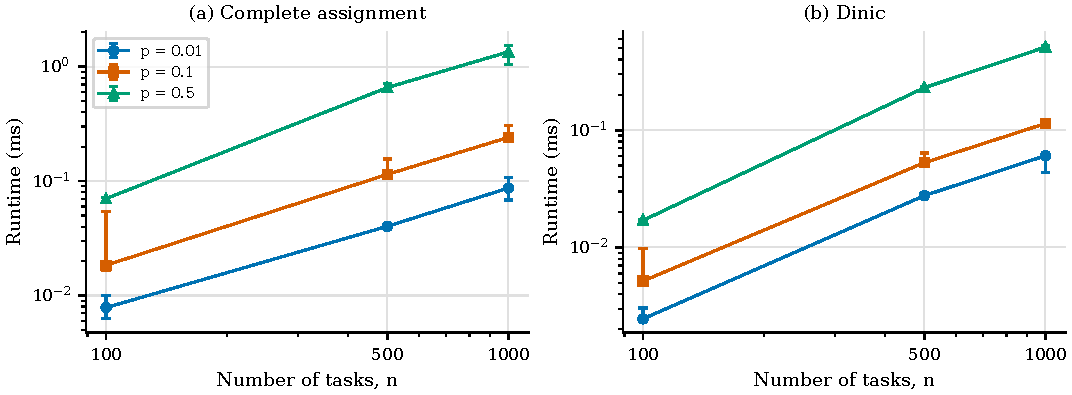
\includegraphics[width=\textwidth]{output/pdf/01_runtime_vs_tasks.pdf}
\caption{Runtime versus task count with $m=100$ and fixed server capacity four.
Each series holds $p$ fixed. Panels show complete assignment time and Dinic time.
Points are medians of three per-seed medians; error bars span their full range.
Both axes are logarithmic.}
\label{fig:tasks}
\end{figure*}

\begin{figure*}[t]
\centering
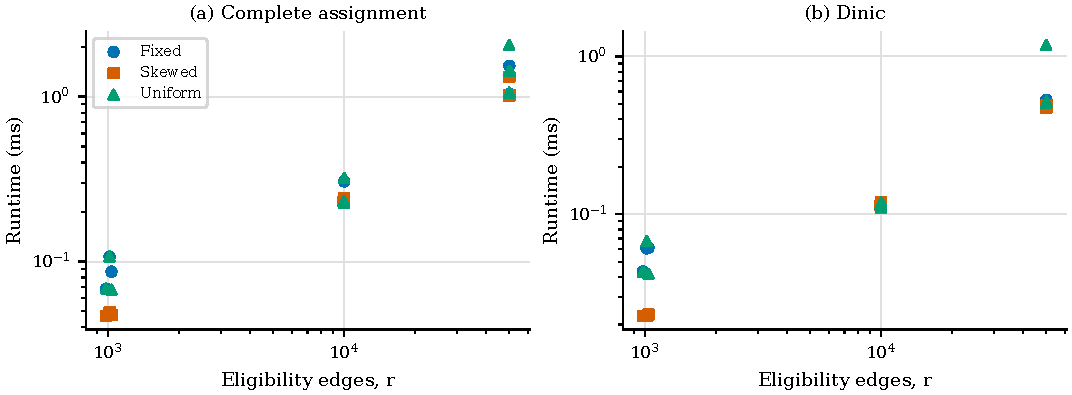
\includegraphics[width=\textwidth]{output/pdf/02_runtime_vs_edges.pdf}
\caption{Runtime versus observed eligibility edges with $n=1000$, $m=100$,
and base capacity four. Each point is one instance's median over nine runs.
Colors and symbols distinguish capacity distributions. Edge counts vary through
$p\in\{0.01,0.1,0.5\}$; no interpolated or simulated timings are plotted.
Both axes are logarithmic.}
\label{fig:edges}
\end{figure*}

\begin{figure*}[t]
\centering
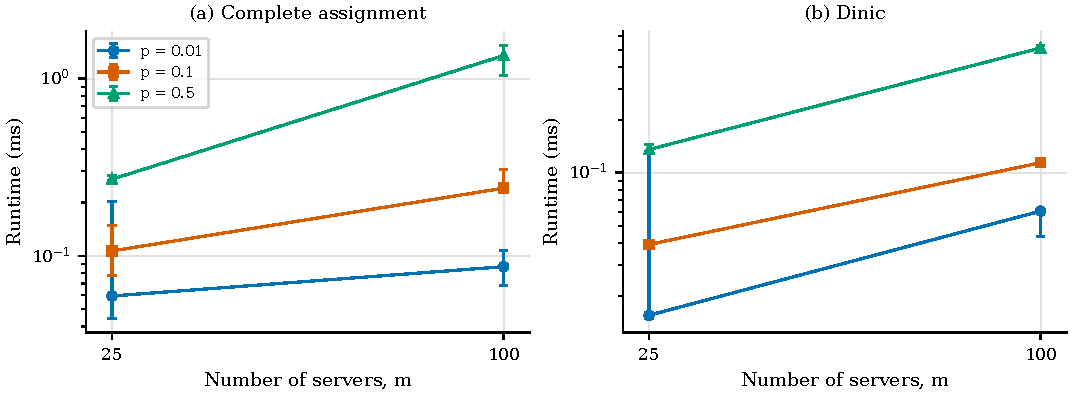
\includegraphics[width=\textwidth]{output/pdf/03_runtime_vs_servers.pdf}
\caption{Runtime versus server count at $n=1000$ and fixed capacity four per
server. Each series holds $p$ fixed. Points show medians across three seed
medians, with their full range. Only two server counts are measured; connecting
segments are visual guides. Runtime axes are logarithmic.}
\label{fig:servers}
\end{figure*}

\begin{figure*}[t]
\centering
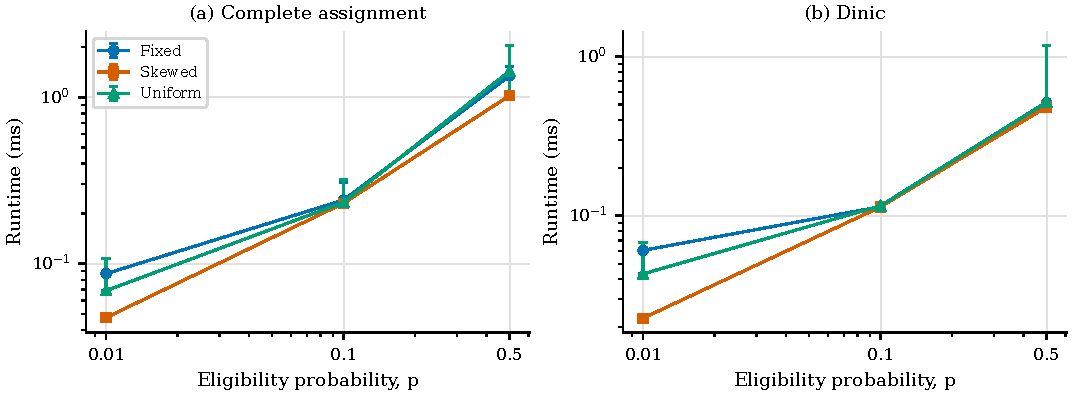
\includegraphics[width=\textwidth]{output/pdf/04_runtime_vs_density.pdf}
\caption{Runtime versus eligibility probability at $n=1000$, $m=100$, and
base capacity four. Capacity distributions have equal expected per-server
capacity but unequal realized aggregate capacity. Points show medians across
three seed medians; error bars span their full range. Both axes are logarithmic.}
\label{fig:density}
\end{figure*}

\begin{figure*}[t]
\centering
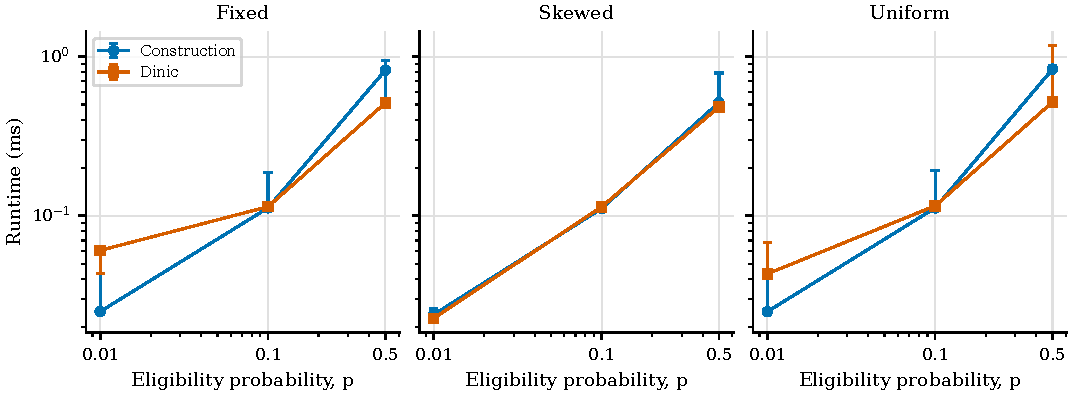
\includegraphics[width=\textwidth]{output/pdf/05_construction_vs_dinic.pdf}
\caption{Network construction and Dinic time at $n=1000$, $m=100$, and base
capacity four, separated by capacity distribution. Construction includes residual
edges and algorithm work arrays. Points show medians across three seed medians;
error bars span their full range. All panels share the runtime scale, and both
axes are logarithmic. Extraction is included in total time but not in these
two component series.}
\label{fig:components}
\end{figure*}

\begin{figure}[t]
\centering
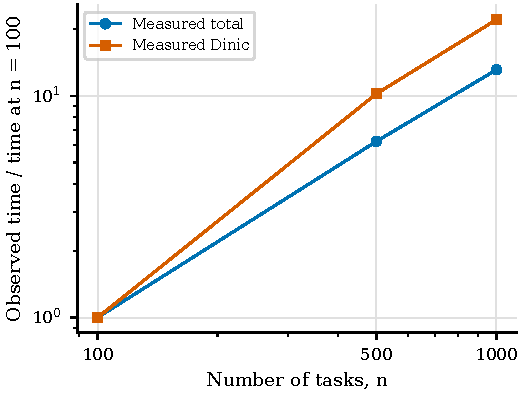
\includegraphics[width=\columnwidth]{output/pdf/06_observed_growth.pdf}
\caption{Observed runtime growth relative to $n=100$, with $m=100$, $p=0.1$,
and fixed capacity four. Each time is the median across three instance medians.
Total-time growth is 6.23 and 13.12 at $n=500$ and 1,000; Dinic-time growth
is 10.22 and 22.06. For comparison in the text, the median $V^2E$ expression
grows by 41.04 and 274.19. Only measured timing ratios are plotted.}
\label{fig:growth}
\end{figure}
